\documentclass{beamer}
%\documentclass[handout]{beamer}
\usepackage{etex}
\usepackage[utf8]{inputenc}
\usepackage[T1]{fontenc}
\usepackage[ngerman]{babel}
\usepackage{color}
\usepackage{colortbl}
\usepackage{amsmath}
\usepackage{amsfonts}
\usepackage{amssymb}
\usepackage{mathabx}
\usepackage{textcomp}
\usepackage{natbib}
\usepackage{multirow}
\usepackage{nicefrac}
\usepackage{multicol}
\usepackage{url}
\usepackage{gb4e-}
\usepackage{pifont}

\title[Topikmodellierung und -domänen]{Induktive Topikmodellierung\\und extrinsische Topikdomänen}
\author[Felix Bildhauer, Roland Schäfer]{Felix Bildhauer$^1$ und Roland Schäfer$^2$}
\institute[]{$^1$Abt.\ Grammatik IDS Mannheim, $^2$Ling.\ Webcharakterisierung (DFG) FU Berlin}
\date[]{IDS Jahrestagung 2016, Mannheim}

\usetheme{Madrid}
\usecolortheme{crane}

\newcommand*\rot{\rotatebox{90}}

\begin{document}

%\titlegraphic{\includegraphics[width=0.2\textwidth]{fulogo}\hspace{0.05\textwidth}
\includegraphics[width=0.125\textwidth]{dfglogo}\hspace{0.25\textwidth}
\includegraphics[width=0.2\textwidth]{idslogo}}
%\frame{\titlepage}

\begin{frame}
%\begin{textblock*}%{2cm}(.35cm,-8cm)                                                                                          
%  \includegraphics[scale=.48]{hukombi_bwb}
\includegraphics[width=0.25\textwidth]{fulogo}\hspace{0.05\textwidth}
\includegraphics[width=0.10\textwidth]{dfglogo}\hspace{0.4
\textwidth}
\includegraphics[width=0.2\textwidth]{idslogo}
%  \end{textblock*}
  \maketitle
\end{frame}



\begin{frame}
  {Hintergrund}
  \begin{itemize}
    \item \alert{Textklassifikation} als \alert{Metadaten} für sehr große Korpora
    \item \alert{Kovariation} grammatischer, lexikalischer und externer Merkmale
    \item \alert{Korpusevaluation} und Korpusvergleich\\
      \citep{Kilgarriff2001,BiemannEa2013,SchaeferBildhauer2013de}
      \vspace{0.5cm}
    \item linguistischer Wunsch nach \alert{Interpretierbarkeit}
      \vspace{0.5cm}
    \item schlechte Qualität bei automatischer Auszeichnung\\
      komplexer Genre- und Register-Kategorien \citep{BiberEgbert2016}
  \end{itemize}
\end{frame}

\begin{frame}
  {COWCat}
  \begin{itemize}
    \item Textklassifikationsschema mit möglichst einfachen Kategorien
    \item keine komplexen Kategorien wie Genres, Register usw.
    \item \textit{Autorschaft}, \textit{Äußerungsabsicht}, \textit{Äußerungsmodus}, \alert{\textit{Topikdomäne}}
      \vspace{0.5cm}
    \item Basis für automatische Klassifikationsversuche
      \vspace{0.5cm}
    \item \cite{Sharoff2006,SchaeferBildhauer2012a}\\
      {\footnotesize \url{http://corporafromtheweb.org/cowcat-categorization-scheme/}}
  \end{itemize}
\end{frame}

\begin{frame}
  {Korpora und Goldstandards}
  \begin{itemize}
    \item DECOW14A: 17 Mrd.\ Wörter Webdaten\\
      \citep{SchaeferBildhauer2012a,SchaeferBildhauer2013de,Schaefer2015b}
    \item DeReKo: 28 Mrd.\ Wörter überwiegend Zeitungstexte\\
      \citep{KupietzEa2010}
      \vspace{0.5cm}
    \item aus beiden Korpora: manuell annotierte Goldstandards\\
      für Topikdomänen mit ca.\ 850 Dokumenten
      \vspace{0.5cm}
    \item {\footnotesize Dank an unsere AnnotatorInnen Sarah Dietzfelbinger, Lea Helmers, Theresia Lehner, Kim Maser, Samuel Reichert, Luise Rißmann (FU Berlin); Monica Fürbacher (IDS Mannheim)}
  \end{itemize}
\end{frame}

\begin{frame}
  {Verteilung der Topikdomänen}
  Wie ähnlich sind sich die beiden Korpora?\\[1cm]
  \begin{center}
    
\includegraphics[width=0.45\textwidth]{dereko}~
\includegraphics[width=0.45\textwidth]{cow}
  \end{center}
\end{frame}

\begin{frame}
  {Topikmodellierung}
  \begin{itemize}
    \item Ziel: \alert{unüberwachte Induktion von Topiks}
    \item Ausgangspunkt der Induktion: Term-Dokument-Matrix
    \item Dokumente gewichtet den Topiks zugeordnet
    \item Topiks definiert durch gewichtete Wörter
    \item Gegensatz zu a priori gegebenen Taxonomien:\\
      nicht strittig und nicht diskret
      \pause
      \vspace{0.5cm}
    \item z.\,B.\ Latent Semantic Indexing \citep{LandauerDumais1994},\\
      Latent Dirichlet Allocation \citep{BleiEa2003}
      \vspace{0.5cm}
    \item für unser Experiment: LSI (Gensim; \citealp{RehurekSojka2010})
  \end{itemize}
\end{frame}

\begin{frame}
  {Topiks auf Topikdomänen abbilden}
  
  Idee\\
  
  \begin{itemize}
    \item Fundierung und Optimierung oft umstrittener\\
      gegebener Klassifikationsschemata (Topikdomänen)\\
      anhand lexikalischer Verteilungen in den Texten
      \vspace{0.25cm}
    \item gewichtete Zuordnung der Dokumente zu Topiks\\
      als Grundlage für \alert{überwachtes Lernen von Topikdomänen}
  \end{itemize}

  Experimente\\
  
  \begin{itemize}
    \item identische Vorverarbeitung (COW-Toolchain)
    \item Ausfilterung schwach repräsentierter Kategorien
    \item Stapeltests mit verschiedenen Klassifikatoren
  \end{itemize}

\end{frame}

%\begin{frame}
%  {Ergebnisse}
%  COW ($\kappa$)\\
%
%  \begin{center}
%    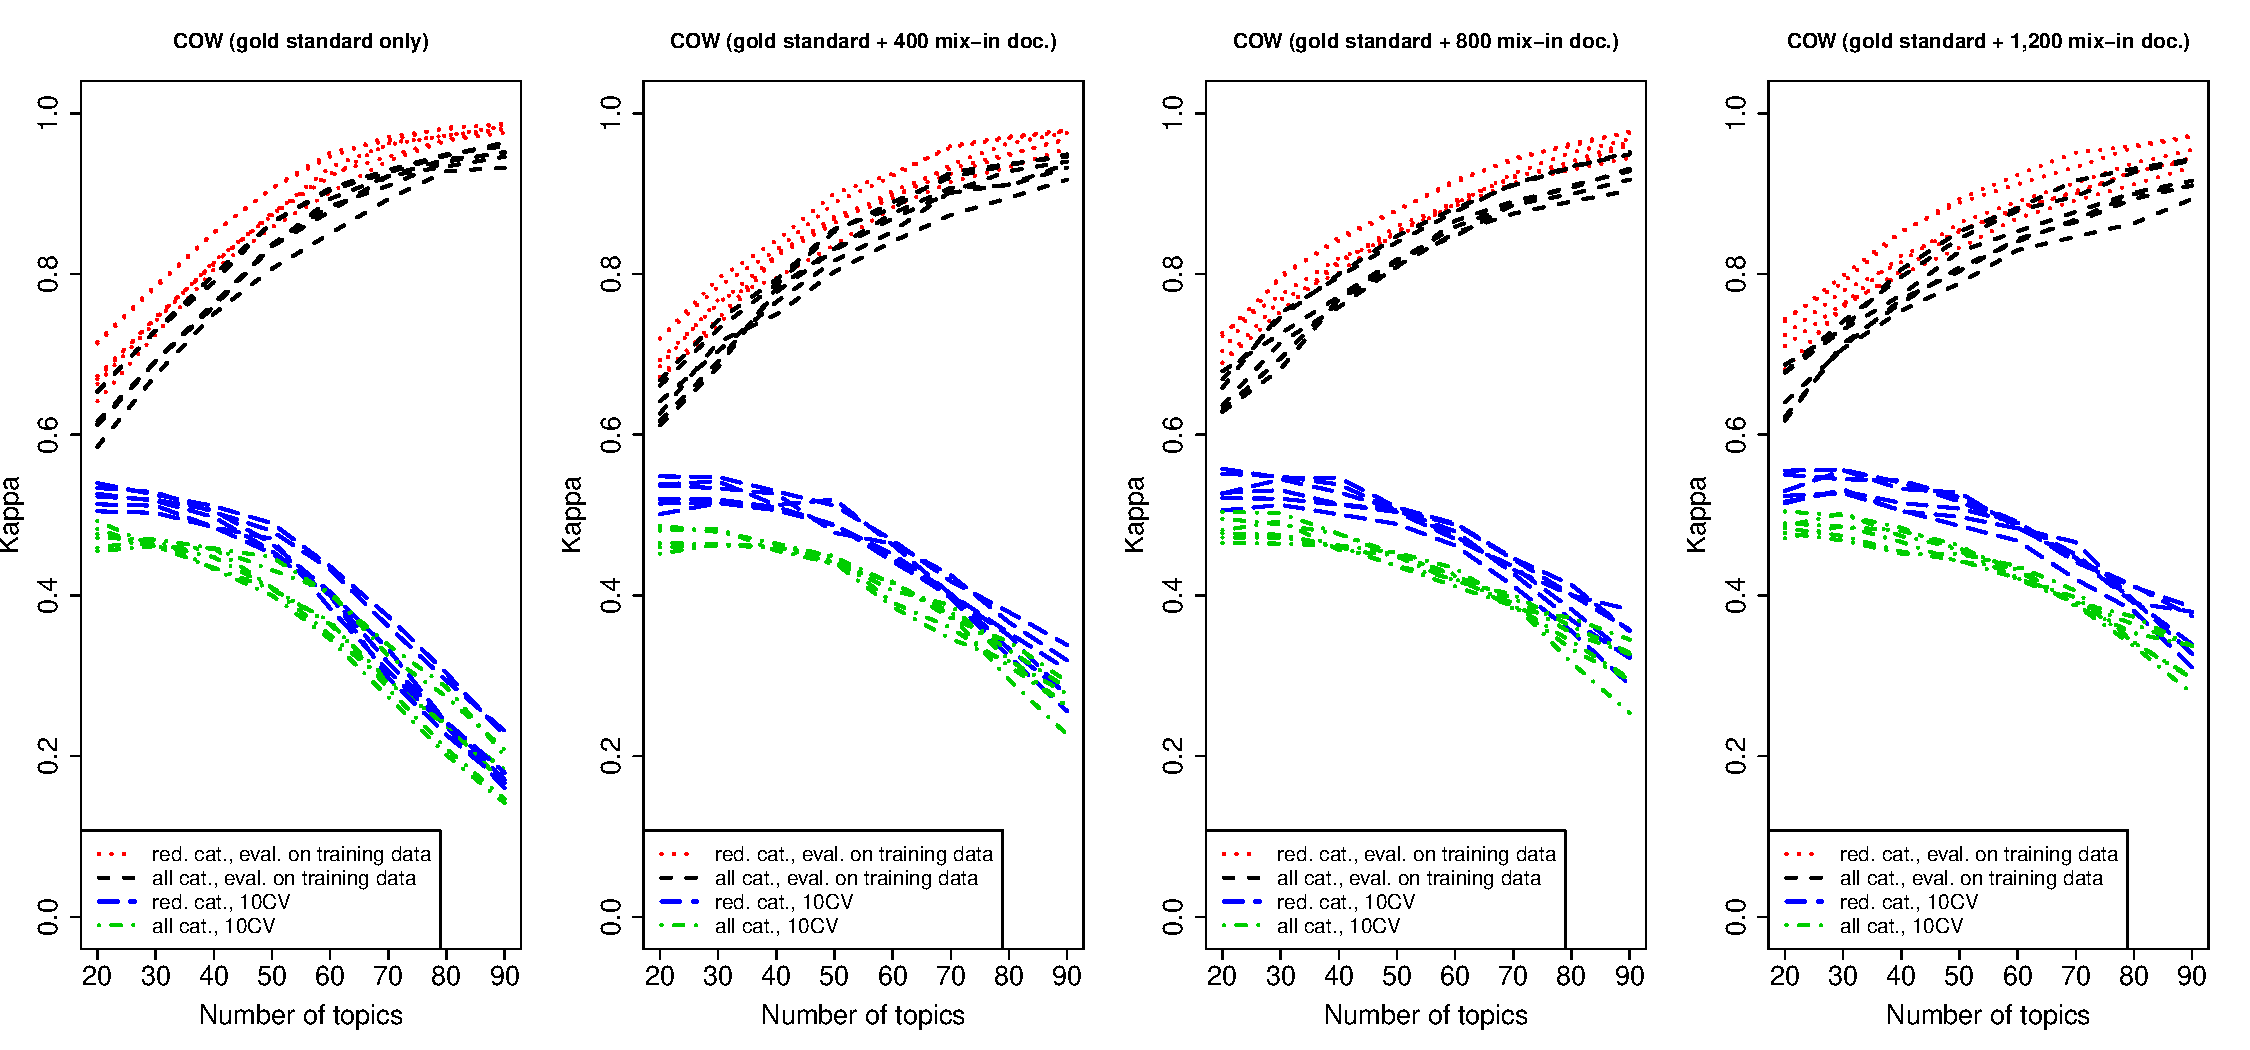
\includegraphics[width=\textwidth]{cow_kappa}
%  \end{center}
%\end{frame}
%
%\begin{frame}
%  {Ergebnisse}
%  DeReKo ($\kappa$)\\
%
%  \begin{center}
%    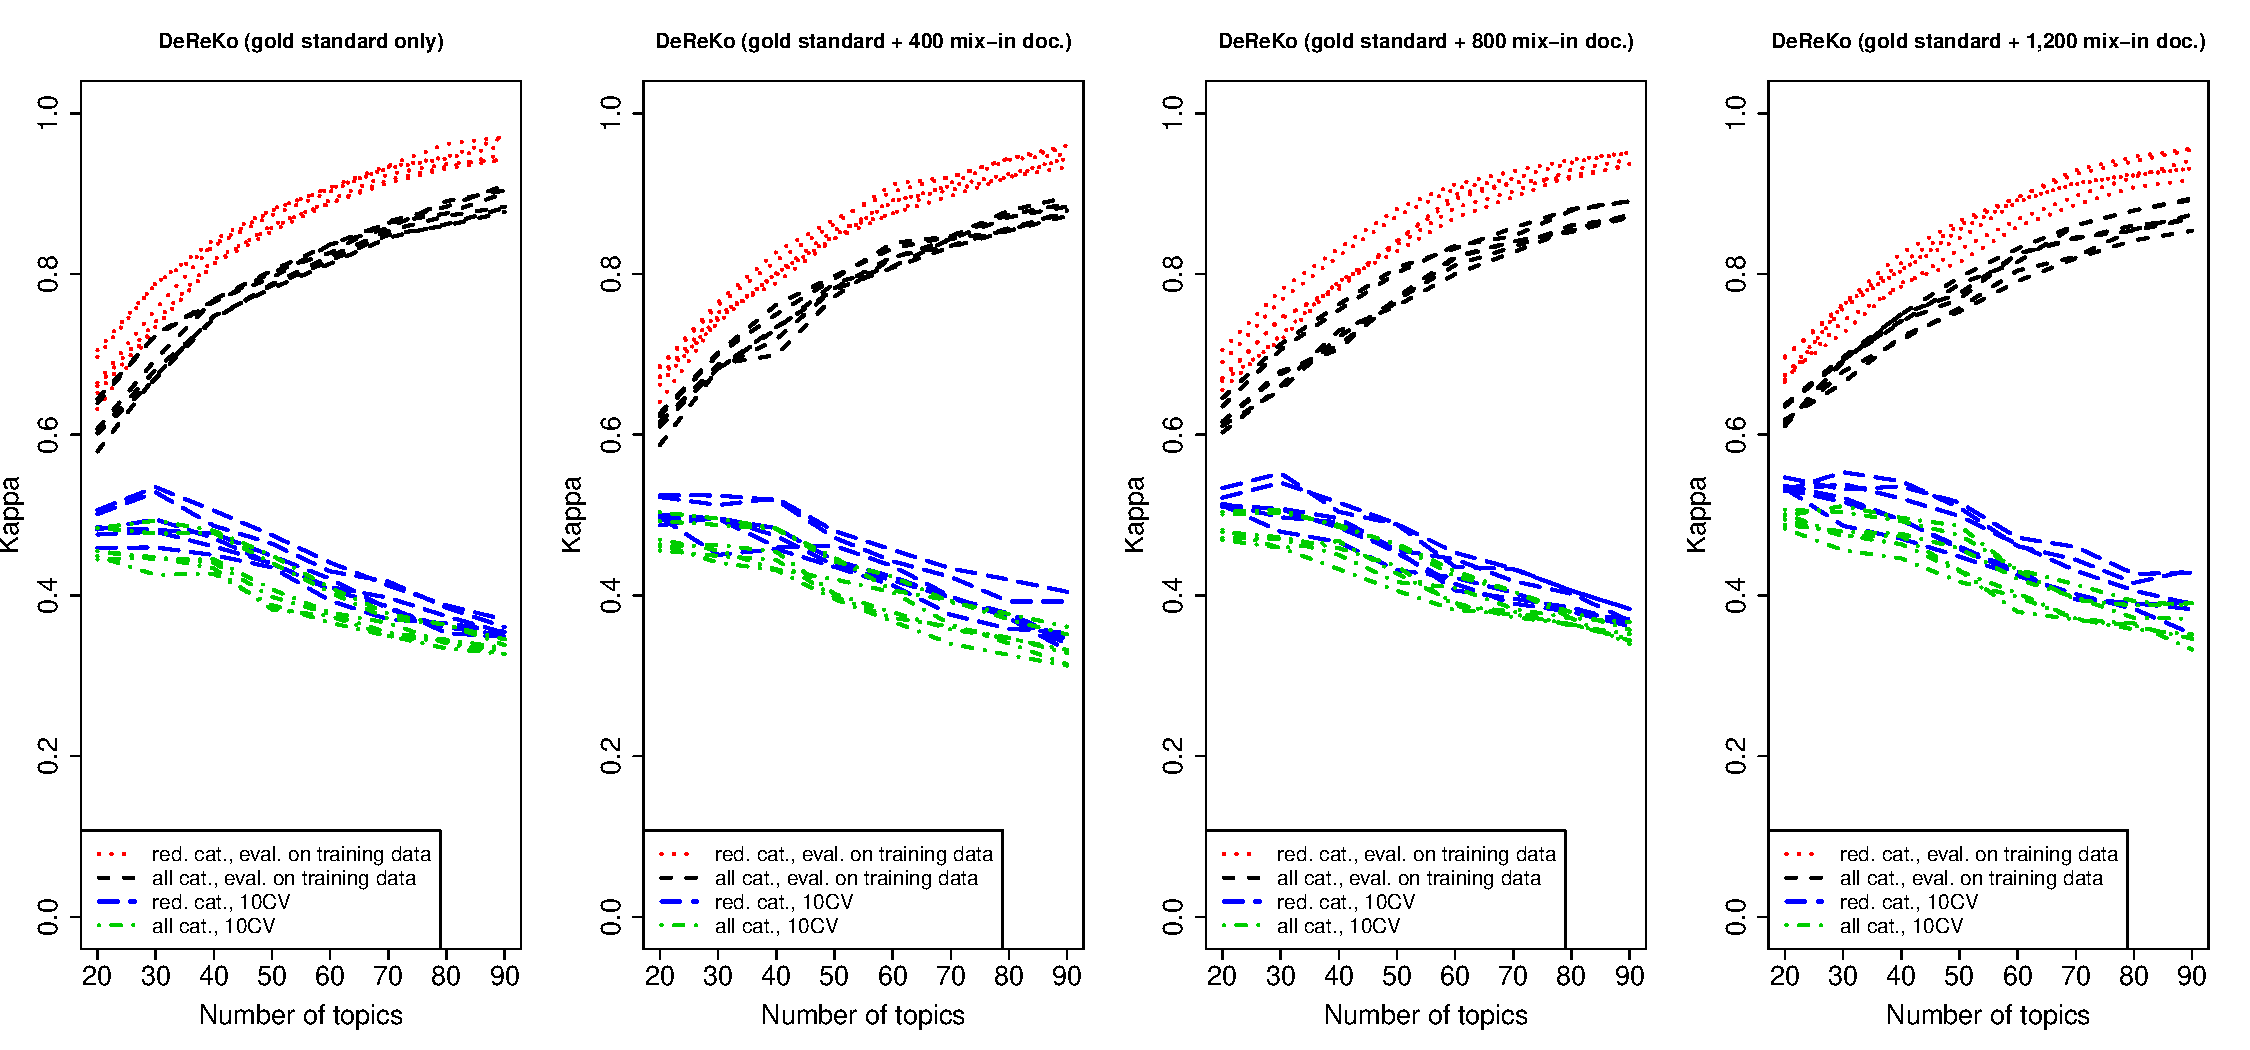
\includegraphics[width=\textwidth]{dereko_kappa}
%  \end{center}
%\end{frame}
%
%\begin{frame}
%  {Ergebnisse}
%  Zusammen ($\kappa$)\\
%
%  \begin{center}
%    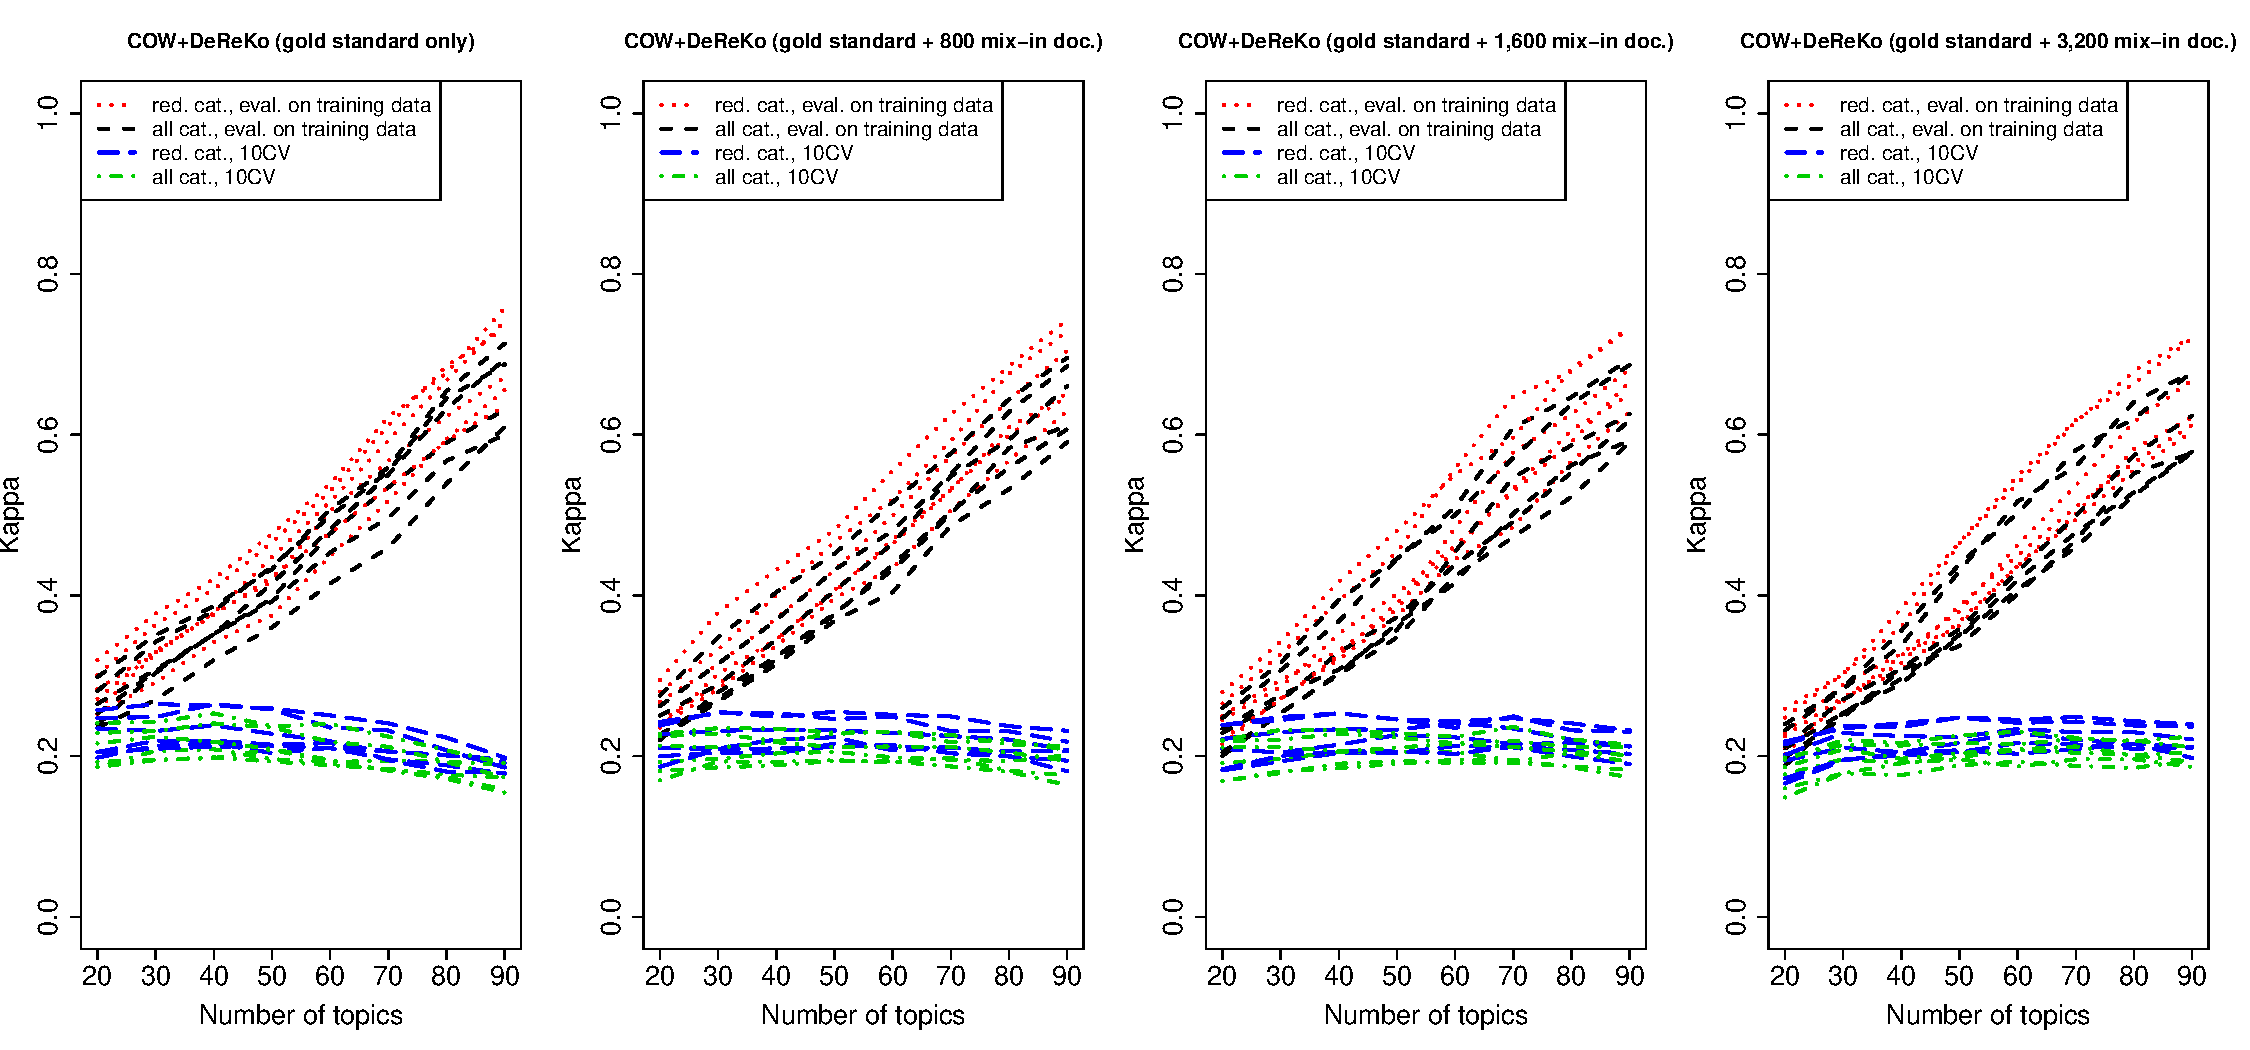
\includegraphics[width=\textwidth]{coreko_kappa}
%  \end{center}
%\end{frame}

\begin{frame}
  {Ergebnisse und Probleme}
  Evaluation\\

  \vspace{0.5cm}
  \resizebox{\textwidth}{!}{\begin{tabular}{lrrrr}
    \hline
    \textbf{Corpus} & \textbf{Accuracy} & \textbf{Precision} & \textbf{Recall} & \textbf{F-Measure} \\
    \hline
    COW &  \alert<2->{68.765\%} & 0.688 & 0.688 & 0.674 \\
    DeReKo & \alert<3->{72.999\%} & 0.725 & 0.730 & 0.696 \\
    COW + DeReKo & \onslide<4->{\alert{?}} & \onslide<4->{?} & \onslide<4->{?} & \onslide<4->{?} \\ 
    \hline
  \end{tabular}}
  \onslide<7->{~}
%  \vspace{0.5cm}
%  Diffusionsmatritzen\\
%
%  \vspace{0.5cm}
%  \resizebox{0.33\textwidth}{!}{\begin{tabular}{|llcccccccc|}
%    \hline
%    \multicolumn{2}{|c}{\textbf{COW}} & \multicolumn{8}{c|}{\textbf{Classified}} \\
%     && \rot{\textbf{PolSoc~}} & \rot{\textbf{Busi}} & \rot{\textbf{Life}} & \rot{\textbf{Arts}} & \rot{\textbf{Public~}} & \rot{\textbf{Law}} & \rot{\textbf{Beliefs~}} & \rot{\textbf{Hist}} \\
%   \hline
%   \multirow{8}{*}{\rot{\textbf{Annotated}}} & \textbf{PolSoc}  & \textbf{26} &  12 &  10 &   1 &   1 &   0 &   1 &   0 \\ 
%     & \textbf{Busi}    &  5 & \textbf{105} &  40 &   7 &   1 &   2 &   1 &   1 \\ 
%     & \textbf{Life}    &  3 &  14 & \textbf{286} &   6 &   4 &   1 &   1 &   1 \\ 
%     & \textbf{Arts}    &  3 &   2 &  36 &  \textbf{78} &   1 &   0 &   2 &   6 \\ 
%     & \textbf{Public}  &  0 &   3 &  11 &   0 &   \textbf{9} &   1 &   0 &   0 \\ 
%     & \textbf{Law}     &  3 &   9 &   8 &   0 &   1 &   \textbf{8} &   0 &   0 \\ 
%     & \textbf{Beliefs} &  4 &   3 &  11 &   6 &   1 &   0 &  \textbf{30} &   1 \\ 
%     & \textbf{Hist}    &  9 &   0 &   9 &   7 &   1 &   1 &   2 &  \textbf{15} \\ 
%     \hline
% \end{tabular}}~~\resizebox{0.25\textwidth}{!}{\begin{tabular}{|llcccccc|}
%    \hline
%     \multicolumn{2}{|c}{\textbf{DeReKo}} & \multicolumn{6}{c|}{\textbf{Classified}} \\
%     && \rot{\textbf{PolSoc~}} & \rot{\textbf{Busi}} & \rot{\textbf{Life}} & \rot{\textbf{Indiv}} & \rot{\textbf{Arts}} & \rot{\textbf{Public}} \\
%    \hline
%     \multirow{6}{*}{\rot{\textbf{Annotated}}}& \textbf{PolSoc}  & 223 & 6 & 39 &  0 &  0 &  8 \\
%     & \textbf{Busi}    &  20 & 24 &   9 &  0 &  0 &  0 \\
%     & \textbf{Life}    &  24 &  1 & 324 &  0 &  0 &  1 \\
%     & \textbf{Indiv}   &   5 &  0 &  17 &  0 &  0 &  1 \\
%     & \textbf{Arts}    &   2 &  0 &  28 &  0 &  6 &  0 \\
%     & \textbf{Public}  &  35 &  0 &  30 &  0 &  0 & 34 \\
%    \hline
% \end{tabular}}~~\resizebox{0.315\textwidth}{!}{\begin{tabular}{|llccccccccc|}
%    \hline
%     \multicolumn{2}{|c}{\textbf{Joint}} & \multicolumn{9}{c|}{\textbf{Classified}} \\
%     && \rot{\textbf{PolSoc~}} & \rot{\textbf{Busi}} & \rot{\textbf{Medical~}} & \rot{\textbf{Life}} & \rot{\textbf{Arts}} & \rot{\textbf{Public~}} & \rot{\textbf{Law}} & \rot{\textbf{Beliefs~}} & \rot{\textbf{Hist}} \\
%    \hline
%    \multirow{9}{*}{\rot{\textbf{Annotated}}} & \textbf{PolSoc}   & \textbf{199} &   7 &   0 & 109 &   0 &  12 &   0 &   0 &   0 \\ 
%    & \textbf{Busi}     &  18 &  \textbf{23} &   0 & 172 &   0 &   2 &   0 &   0 &   0 \\ 
%    & \textbf{Medical}  &   6 &   0 &   \textbf{0} &  29 &   0 &   1 &   0 &   0 &   0 \\ 
%    & \textbf{Life}     &  25 &   4 &   0 & \textbf{632} &   0 &   5 &   0 &   0 &   0 \\ 
%    & \textbf{Arts}     &   2 &   2 &   0 & 160 &   \textbf{0} &   0 &   0 &   0 &   0 \\ 
%    & \textbf{Public}   &  46 &   2 &   0 &  56 &   0 &  \textbf{19} &   0 &   0 &   0 \\ 
%    & \textbf{Law}      &   8 &   0 &   0 &  31 &   0 &   0 &   \textbf{0} &   0 &   0 \\ 
%    & \textbf{Beliefs}  &   0 &   0 &   0 &  59 &   0 &   0 &   0 &   \textbf{0} &   0 \\ 
%    & \textbf{Hist}     &   4 &   0 &   0 &  50 &   0 &   0 &   0 &   0 &   \textbf{0} \\ 
%    \hline
% \end{tabular}}

\end{frame}

%\begin{frame}
%  {Aktuell}
%  Was die Ergebnisse nahelegen\dots\\
%
%  \vspace{0.5cm}
%
%  \begin{itemize}
%    \item größere Goldstandards
%    \item Aufteilen überstark repräsentierter Kategorien
%    \item im Projekt \textit{linguistische Webcharakterisierung} (FU Berlin):\\
%      5000 Goldstandard-Dokumente angestrebt
%      \vspace{0.5cm}
%
%    \item<2-> Aber: \alert{Brauchen wir wirklich interpretierbare Kategorien?}
%  \end{itemize}
%\end{frame}

% --------------- REFS + APPENDIX

\begin{frame}[allowframebreaks]
  {References}
  \def\newblock{\hskip .11em plus .33em minus .07em}
  \footnotesize
  \bibliographystyle{abbrvnat} 
  \bibliography{coreko}
\end{frame}

\end{document}
